\documentclass{article}
\usepackage{graphicx} % Required for inserting images
\usepackage[a4paper, total={6in, 8in}]{geometry}

% to make itemizes take less space
\usepackage{enumitem}% http://ctan.org/pkg/enumitem
\graphicspath{ {./images/} }

% Tables
\usepackage{booktabs}
\usepackage{longtable}
\usepackage[normalem]{ulem}
\useunder{\uline}{\ul}{}


\title{GPIG-A Formative}
\begin{document}
\maketitle

\section{An outline of the proposed technical solution}

We are concerned with the growth of destructive plants within a forest, these are plants who outcompete their neighbours, make extinct other plants, reduce biodiversity, and alter habitats. 
We propose a solution that uses drones to monitor and capture image data of a given forest, each image is handed back to a central system where we identify the plants present in the image, and store that along with the latitude and longitude.
This system is generic enough to work in any forest, but has the option to train it against specific plants that you are concerned about, such that it can give deeper insights and recommendations.
Our user interface allows an operator to:
\begin{itemize}[noitemsep,topsep=3pt]
\item See the locations of each drone,
\item See which areas have most recently been scanned,
\item Chat with a large language model about the data obtained.
\item See the growth of plant species over time
\end{itemize}


The plants within each captured image will be clustered such that similar looking plants are given the same ID. 
By tracking the quantity of each identified plant over time, we can see if any are undergoing exponential growth.
For each plant species $s$ that we are especially concerned with, we allow the training of a plant classification module $f(I) \rightarrow [0,1]$ mapping a series of images $I$, belonging to a given id onto the probability that they are of species $s$. 
This would allow us reasonable confidence that our plant id maps to a given species.
We can then use this to make more informed recommendations.

Using a button on our user interface, this data will get wrapped into a pre-made prompt that can then be sent to a large language model.
The pre-made prompt would say which plants are growing and where, the drone scan history, the location of the forest, and the predicted plant name (if we have it), and would ask for advice on how to handle it.
The operator can have a conversation with the large language model where they try to plot the best course of action going forward.

\section{A brief description of the system that will be prototyped (including assumptions, capabilities, primary functions)}

\begin{figure}[htbp]
    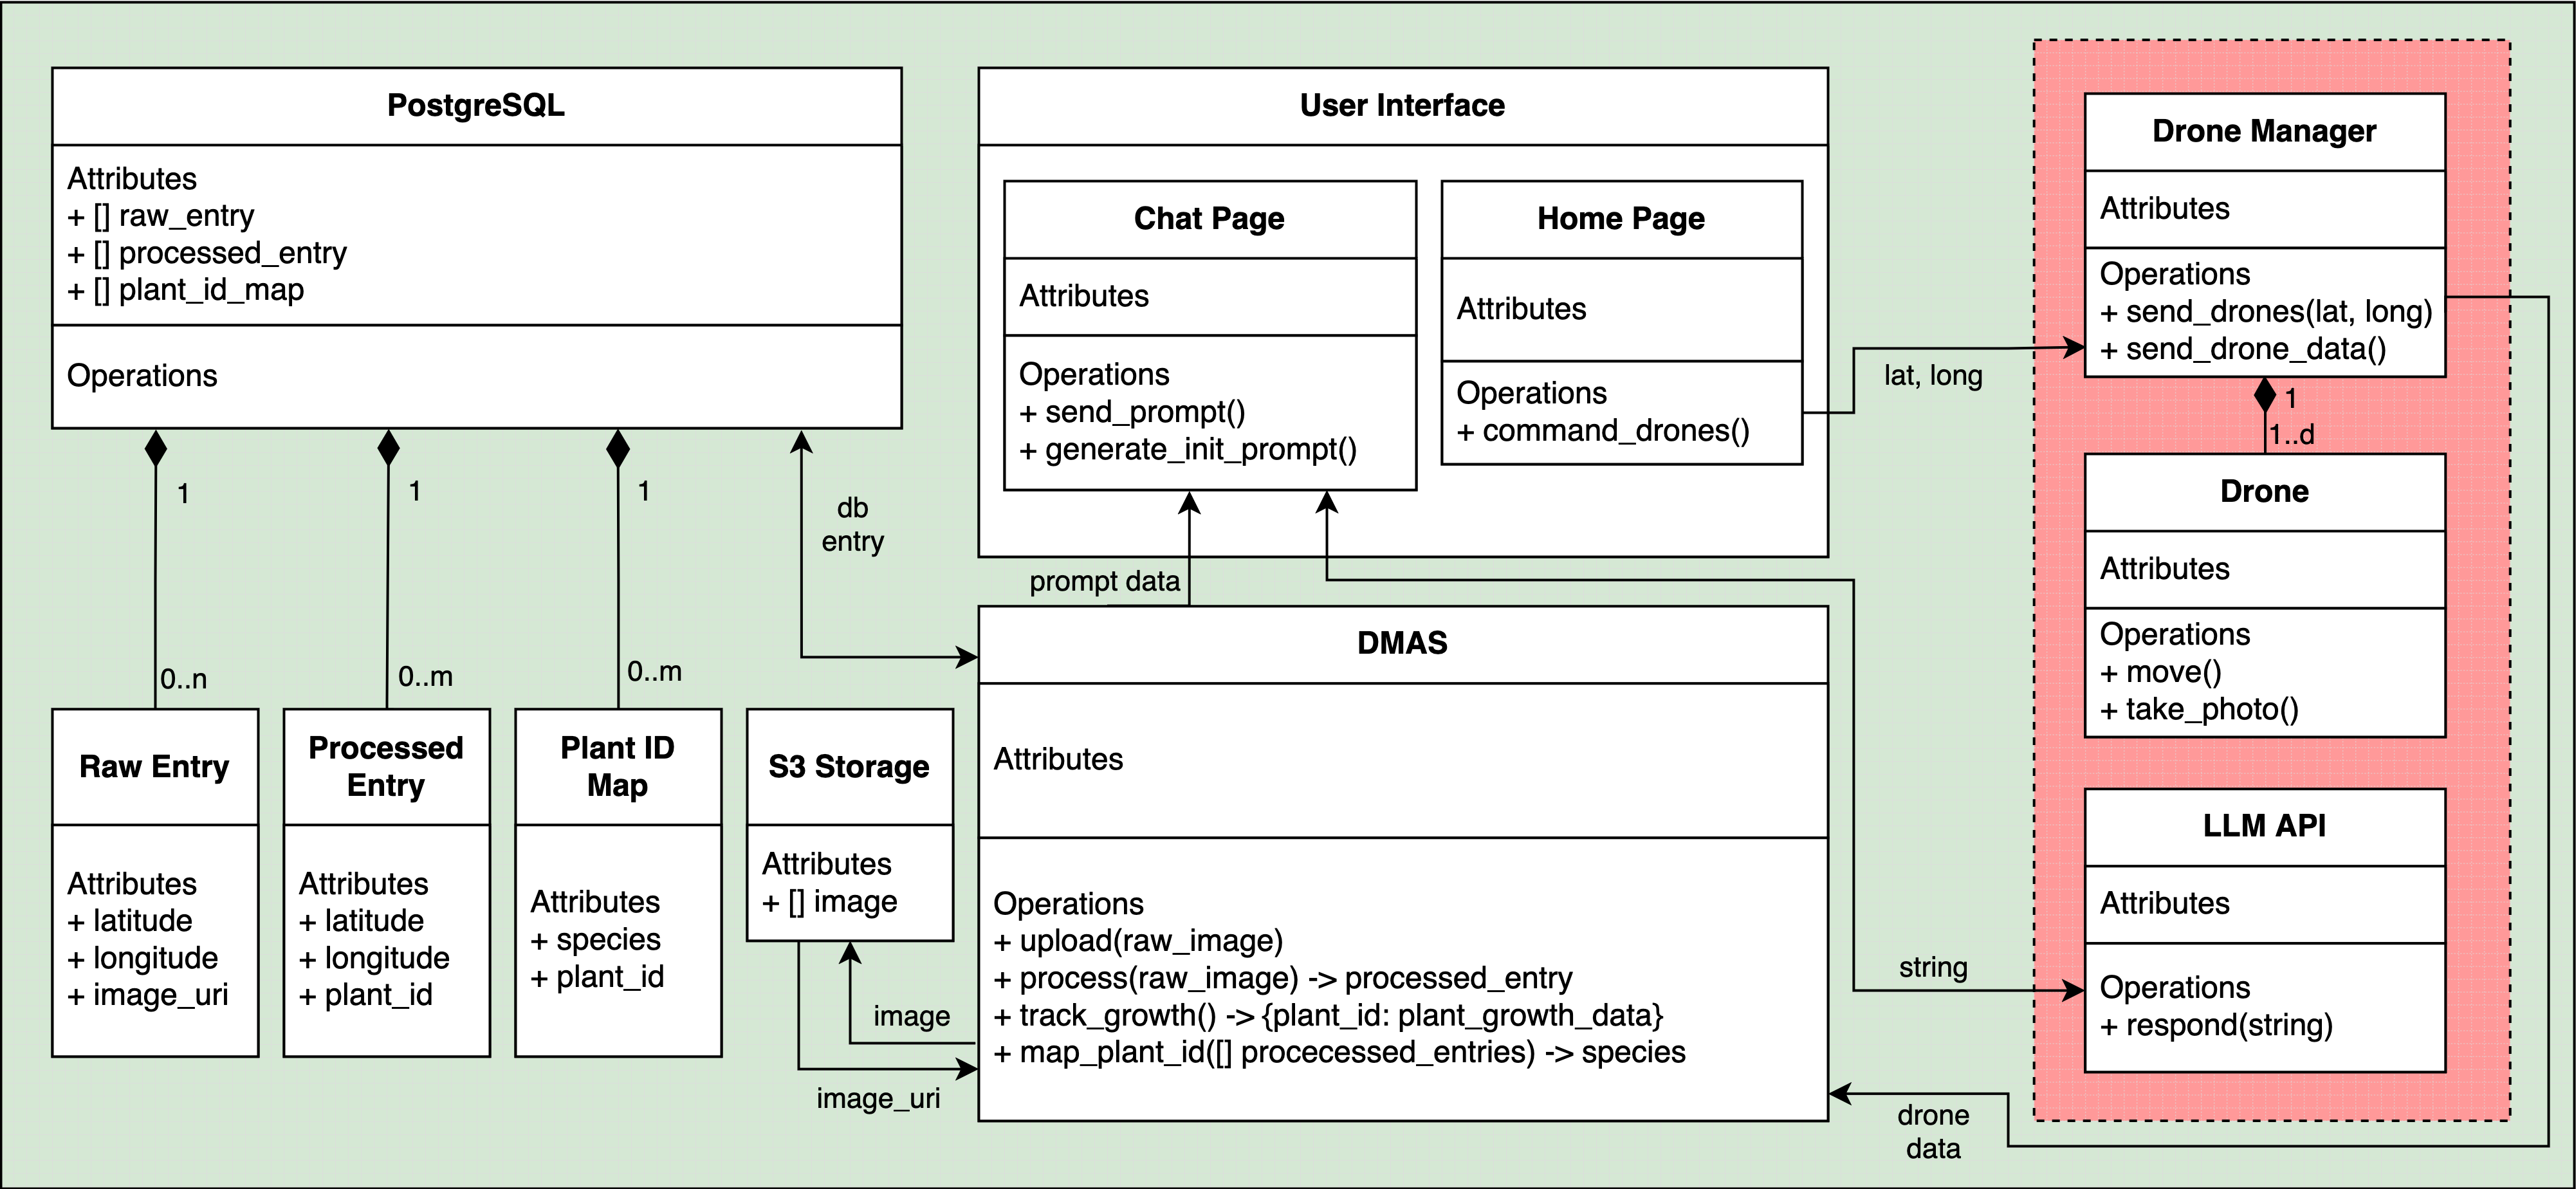
\includegraphics[width=\textwidth]{block_diagram}
    \caption{The block diagram of our microservices.  \\ 
    Key: Green = will implement, Red = will mock/simulate}
    \label{fig:design}
\end{figure}

% TODO, not really sure how to talk about assumptions, capabilities, and primary functions. I have done my best but this could definitely do with some major work.

As you can see in fig. \ref{fig:design}, the following systems will be present in our prototype:
\begin{itemize}[noitemsep,topsep=3pt]
\item The datastore and data analysis,
\item The plant clustering and id assignment,
\item An example plant classifier module,
\item The user interface,
\item Drone simulation,
\item Large language model communication.
\end{itemize}

\noindent
The datastore will be a PostgreSQL database containing gour tables:
\begin{itemize}[noitemsep,topsep=3pt]
\item Raw image entries containing columns for latitude, longitude, camera pose, and the corresponding image URI,
\item Processed entries containing columns for latitude, longitude, and plant id,
\item A map from plant id to species, 
\item Drone location history entries.
\end{itemize}
We assume that this is sufficient for the final product.

% This paper is due in april, I suspect that we will know by then so maybe this will need changing in the future. 
% TODO Babar should expand on this
We aren't currently sure how exactly we will do the plant clustering and id assignment.
If using k-means clustering we would have to carefully define a value of K for each forest, this wouldn't be ideal as it reduces the adaptability of our system.
We will need to look into clustering techniques that work with variable cluster quantities.
We will have an example plant classifier that, given a cluster of images, predict whether they belong to the species Japanese knotweed, to do this we will need to gather a large number of images of the plant to use as training data. 
We assume that this will be possible. % by the submission of this paper we will likely want to change the tense of this

% TODO Maybe marks and ellie can expand on this
The user interface will be created using react and we will prioritise the functionality over UX/UI design. 

% TODO Maybe Jacob and Jakub can work on this
Drone simulation will be done using ROS2 and Unreal Engine. %TODO Is this correct?
We assume that the code operating the drones in the simulation will work on real drones in a forest, this will need to be tested as simulation can only approximate the real world, there are many factors that we can't account for.

% TODO Maybe Babar and CJ can expand on this
Our large language model communication will be handled as follows: Take the data from our system, format it into a prompt, and forward the response to user interface.
In the final product this could use a specially trained LLM or a fine-tuned LLM, but for our prototype we will hook into GPT-3.5 using their public API % we might not actually use this LLM, change if necessary. 

% TODO Maybe Laura can expand on this
We have containerised our prototype so that functionality is split into microservices, these can be worked on independently by each team.
Each microservice is containerised and the entire project can be run using docker compose.

% TODO maybe we should talk about our sizing estimations, once Prajj has completed his sizing spreadsheet he could talk about it here?

\section{An overview of the system aspects that the team intends to demonstrate in the group}

In our presentation to the customer we intend to demonstrate the following aspects of our system:
\begin{enumerate}[noitemsep,topsep=3pt]
    \item The coordination of drones to scan specific areas, % this might change depending on how much we want to do with drones
    \item A simulation of how our system responds when it discovers that plants are growing destructively,
    \item A conversation with our large language model.
\end{enumerate}

To demonstrate the coordination of our drones we will start at the home page of our user interface where the user is presented with a map. 
The demonstrator will then select an area on the map and the interface will provide a pop up asking if they want to direct the drones to that location, the demonstrator will accept.
The user interface will then show the drones travelling to the new area, and we will show a monitoring web page that shows us tracking the new plants we have discovered.

To demonstrate how our system responds when it discovers that plants are growing destructively, we will restart the system and feed it with a testing data set where one species has been growing exponentially, and is outcompeting its fellow plants.
We will show how the system presents this data to the user and compare it to a situation where the plants do not grow destructively.
This will also demonstrate how we test our system.

To demonstrate a conversation with our large language model we will feed our system the same destructive species test data set but this time the demonstrator will select the button that allows them to have a conversation with a large language model about the results.
We do not plan on implementing the large language model for the prototype, so this will be done by having a pre-generated script.

\section{A summary of progress}

% TODO closer to the deadline of this paper

\section{A brief risk register}

%https://docs.google.com/document/d/118jg7LwiYVXQmANl-qmUPp1iQ2_lbnW4YSJ4lxWL0pY/edit
\begin{longtable}{p{0.2\textwidth}p{0.1\textwidth}p{0.1\textwidth}p{0.4\textwidth}}
    \toprule
    Risk & Likelihood & Effect & Mitigation and Contingency \\ \midrule
    \hline \\
    Team member unavailable for meetings                      & Medium     & Low    & We will host the meeting when the maximum number of team members are available and provide minutes for those who cannot make it.                                                             \\
    Team member unable to complete work                       & Low        & Medium & Deliverables of the projects are assigned to at least two members. We will have stand up meetings to update the team on progress.                                                           \\
    Loss of report                                            & Low        & High   & The report is done in Latex, we will have store this in GitHub and use version control so that we can roll back any mistakes.                                                               \\
    Loss of code                                              & Low        & High   & The code is stored in GitHub, we will use version control so that we can roll back any mistakes.                                                                                            \\
    Team member misunderstands their task                     & Medium     & Medium & We will collaborate when defining what tasks need completing, this means that every member should be aware of what is needed. Having two people per task should also make this less likely. \\
    Team member unavailable for a significant period of time. & Low        & High   & We will reassign tasks to other team members as necessary/based on task importance. We will also inform the module staff about the situation. \\ \bottomrule
    \caption{Risk Register}
    \label{tab:RiskRegister}
\end{longtable}

\end{document}